\section{Stealing a context}
\label{talloc:stealing}

Talloc has the ability to change the parent of a talloc context to another
one. This operation is commonly referred to as stealing and it is one of
the most important actions performed with talloc contexts.

Stealing a context is necessary if we want the pointer to outlive the context it
is created on. This has many possible use cases, for instance stealing a result
of a database search to an in-memory cache context, changing the parent of a
field of a generic structure to a more specific one or vice-versa. The most
common scenario, at least in SSSD, is to steal output data from a function-specific
context to the output context given as an argument of that function -- this is
more deeply explained as one of the best practices in Section 
\ref{talloc:subsec:function-use-own-context}.

\begin{funcproto}
void *talloc_steal(TALLOC_CTX *ctx, const void *ptr)
\end{funcproto}
\begin{funcdesc}
  Changes the parent of the |ptr| to |ctx| and returns |ptr|.
\end{funcdesc}
\begin{funcproto}
void *talloc_move(TALLOC_CTX *ctx, const void **ptr)
\end{funcproto}
\begin{funcdesc}
  Changes the parent of the |ptr| to |ctx| and returns |ptr|.
  Additionally assigns |NULL| into |ptr|.
\end{funcdesc}
\funclistend
In general, the pointer itself is not changed (it only replaces the
parent in the meta data). But the common usage is that the result is assigned
to another variable, thus further accessing the pointer from the original
variable should be avoided unless it is necessary. In this case
|talloc_move()| is the preferred way of stealing a context as it protects the
pointer from being accidentally freed and accessed using the old variable after
its parent has been changed.

\begin{lstlisting}[caption={talloc_steal() and talloc_move()}]
struct foo *foo = talloc_zero(ctx, struct foo);
foo->a1 = talloc_strdup(foo, "a1");
foo->a2 = talloc_strdup(foo, "a2");
foo->a3 = talloc_strdup(foo, "a3");

struct bar *bar = talloc_zero(NULL, struct bar);
/* change parent of foo from ctx to bar */
bar->foo = talloc_steal(bar, foo);

/* or do the same but assign foo = NULL */
bar->foo = talloc_move(bar, &foo);
\end{lstlisting}

\begin{figure}[H]
  \centering
  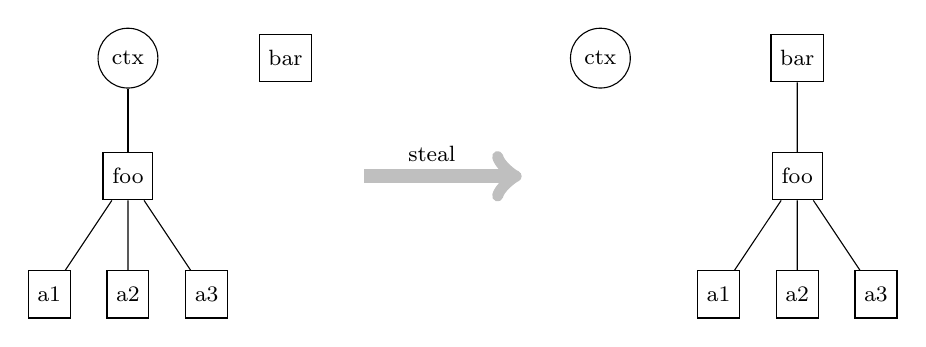
\begin{tikzpicture}
[level/.style={sibling distance=10mm},
 level 1/.style={sibling distance=20mm},
 every node/.style=
   {minimum height=6mm,rectangle,draw=black,font=\footnotesize}]
\begin{scope}
  \node [circle] {ctx}
    child {node [] {foo}
      child {node [] {a1}}
      child {node [] {a2}}
      child {node [] {a3}}
    }
  ;
\end{scope}

\begin{scope}[xshift=2cm]
\node [] {bar};
\end{scope}

\draw [->, line width=5pt, black!25] (3,-1.5) -- 
  node [draw=none,black,yshift=8pt,xshift=-4pt] {steal} (5,-1.5) ;

\begin{scope}[xshift=6cm]
\node [circle] {ctx}
;
\end{scope}

\begin{scope}[xshift=8.5cm]
  \node [] {bar}
    child {node [] {foo}
      child {node [] {a1}}
      child {node [] {a2}}
      child {node [] {a3}}
    }
  ;
\end{scope}
\end{tikzpicture}
  \caption{Stealing a talloc context}
  \label{fig:steal}
\end{figure}
